\documentclass[10pt,a4paper]{article}

\usepackage[utf8]{inputenc}
\usepackage[T1]{fontenc}
\usepackage{amsmath,amssymb,amsfonts}
\usepackage{graphicx}
\usepackage{hyperref}
\usepackage{algorithm}
\usepackage{algpseudocode}
\usepackage{geometry}
\usepackage{cite}

% Page layout
\geometry{margin=1.5cm}

% Title page
\title{\Large\textbf{PixelBytes: Catching Unified Representation for Multimodal Generation}}
\author{\large Fabien Furfaro $^{*}$}
\date{\large 2024}

\begin{document}

\maketitle

\let\thefootnote\relax\footnotetext{$^{*}$ Corresponding author: Fabien Furfaro (\textbf{\href{mailto:fabien.furfaro@gmail.com}{\texttt{fabien.furfaro@capgemini.com}}}).}

\begin{abstract}
This report introduces PixelBytes, a novel approach for unified multimodal representation learning. Inspired by existing sequence models such as Image Transformers, PixelCNN, and Mamba-Bytes, our method aims to capture diverse inputs in a cohesive representation, exploring the integration of different data types, particularly text, audio, and pixelated images (sprites). We conducted our experiments on a specialized PixelBytes Pokémon dataset. Initially, we investigated various model architectures, including Recurrent Neural Networks (RNNs), State Space Models (SSMs), and Attention-based models, focusing on bidirectional processing and our convolutional PxBy embedding technique. Subsequently, we shifted our focus to evaluating models based on data reduction strategies and the effectiveness of autoregressive learning. We specifically examined Long Short-Term Memory (LSTM) networks in both predictive and autoregressive modes for our main experiments. Our findings indicate that autoregressive models outperform predictive models. By adopting a flexible approach to multimodal modeling, PixelBytes aims to support the development of foundation models capable of understanding and generating multimodal data. Code and pretrained models are available at \url{https://github.com/fabienfrfr/PixelBytes} and \url{https://huggingface.co/ffurfaro/aPixelBytes-Pokemon}.
\end{abstract}

\begin{figure}[ht]
\centering
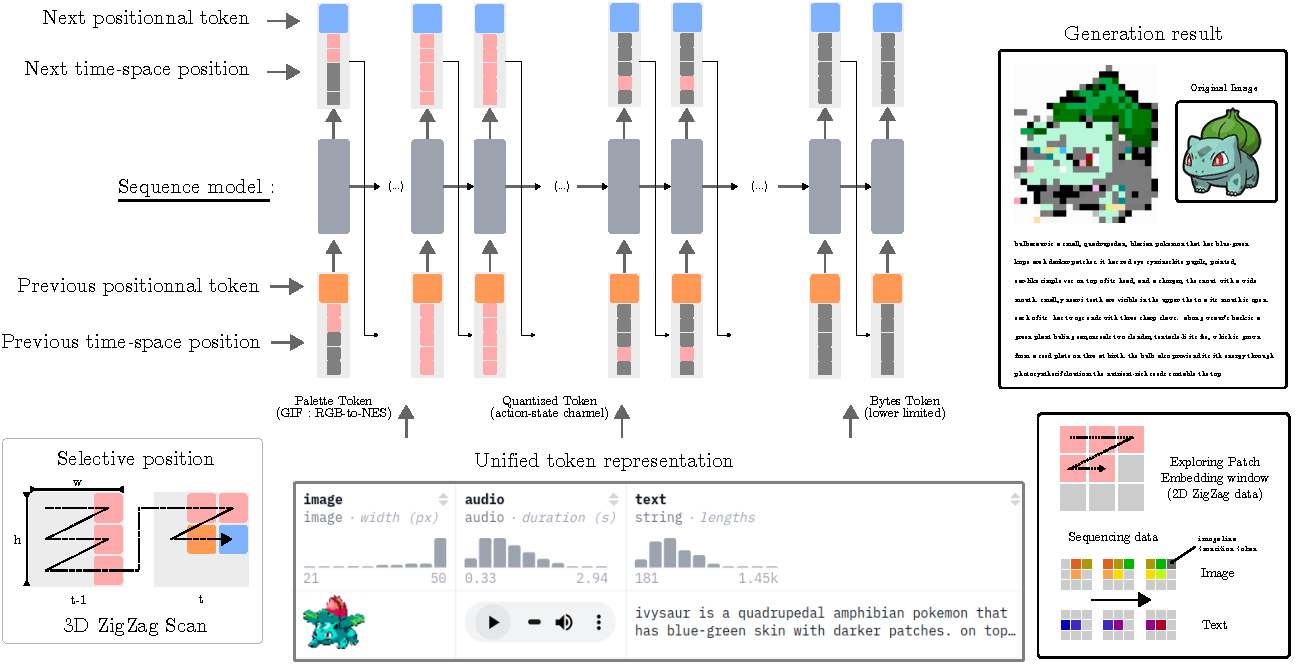
\includegraphics[width=0.8\linewidth]{aPxBy_approach.pdf}
\caption{Overview of the PixelBytes approach: (Left) The scanning process reads different modalities at specific positions. (Center) An example of our dataset and the autoregressive generation across modalities. (Right) A generation example, with the PxBy embedding window displayed below. Note: The model currently shows some inaccuracies in image generation and may produce incorrect words, highlighting areas for future improvement.}
\label{fig:approach_overview}
\end{figure}

\section{Introduction}

Recent advancements in artificial intelligence have led to increasingly generalist models, not by combining multiple specialized components (like Gato from DeepMind \cite{reed2022generalist}), but by giving simple tasks to models where emergent properties—complex behaviors that arise from simpler underlying rules—appear. This is the case with generative language models like GPT \cite{brown2020language}. However, these models are limited by their focus on language alone, failing to capture the full complexity of multimodal understanding \cite{huang2023language}. To address this limitation, researchers have explored combining LLMs with other modalities \cite{liu2024visual}. But this brings us back to the initial problem, as it often results in specialized model combinations without allowing for new emergent properties. We propose "PixelBytes", a novel approach enabling unified training across modalities by capturing diverse inputs in a single, cohesive representation.

Multimodal sequence generation, which involves the creation of coherent outputs combining various data types such as text, images, and numerical sequences, presents a significant challenge in artificial intelligence \cite{baltruvsaitis2018multimodal}. While models like GPT have excelled in text generation \cite{brown2020language}, there's a growing need for unified approaches that can seamlessly handle varied data types. Building upon these findings, PixelBytes aims to address the challenge of unified text, audio and image generation by proposing a model capable of producing mixed sequences of text, audio and images in a coherent and unified manner. We draw inspiration from state-of-the-art sequence models, including Image Transformers \cite{parmar2018image}, PixelCNN \cite{van2016conditional}, and recent developments in bytes generation by mamba architectures \cite{wang2024mambabyte}.

Our research explores various architectures including Recurrent Neural Networks (RNNs), State Space Models (SSMs) \cite{dao2024transformers}, and Attention-based models, focusing on the effectiveness of bidirectional processing \cite{zhu2024vision}, novel embedding techniques (particularly PxBy embedding, which unifies pixel and byte-level representations), the impact of convolutional layers, effects of model depth, input dimensionality, and size. 

Our experiments, conducted on a specialized PixelBytes Pokémon dataset, reveal that autoregressive models with balanced data reduction strategies outperform predictive models in terms of accuracy and loss. While our initial exploration suggested potential for bidirectional sequence models with PxBy embedding and convolutional layers, our final results focus on the performance of Long Short-Term Memory (LSTM) networks in both predictive and autoregressive modes. This paper presents our methodology for constructing unified sequence data from text, audio, and pixelated images (sprites), as well as our experimental results and analysis. By adopting a flexible approach to multimodal modeling, PixelBytes aims to advance the development of versatile foundation models capable of understanding and generating multimodal data.

\section{Exploration for a Unified Representation}

\subsection{Hypothesis Testing Framework}

The quest for a unified data representation across different modalities presents significant challenges. Text data typically has a one-dimensional dependency on preceding words with discrete values \cite{bengio2003neural}. Audio signals, on the other hand, have a temporal dimension with continuous values \cite{van2016wavenet}. Action-state representations in robotics can be similar to audio but with correlations between channels \cite{botteghi2021low}. Images and animations combine spatial and temporal dimensions across discrete RGB channels \cite{krizhevsky2012imagenet}. Given these diverse characteristics, many researchers have focused on combining separate embedding models into a single framework, as seen in projects like ImageBind \cite{girdhar2023imagebind} and RT-2 \cite{zitkovich2023rt}, rather than seeking a truly unified data representation. However, to build a model that comprehensively understands different modalities without intermediate alignment steps, exploring a unified data representation becomes necessary. In this section, we will test several hypotheses:

\begin{itemize}
    \item Can we quantize data such that each element becomes a token? \cite{zhan2022auto}
    \item Is predicting only the next value sufficient for a sequence model to learn effectively?
    \item For dimensions higher than one, is applying a convolutional filter necessary?
    \item For space-time dependency, what is the importance of bidirectionality in models?
\end{itemize}

Through these investigations, we aim to explore a method of representing data that could enable models to understand various types of modalities.

\subsection{Conceptual Multimodal Embedding}

\subsubsection{Dataset Construction}

To test our hypotheses on unified representation, we needed a dataset combining visual and textual data in a format suitable for byte-level processing. Image captioning datasets proved unsuitable due to limited text content and difficulties in interpreting pixelated versions of high-resolution images. We therefore created a specialized Pokémon dataset, offering pixelated designs and rich descriptive text. We collected data by web scraping Pokémon miniatures and descriptions from Pokepedia using Beautiful Soup \cite{richardson2007beautiful}, maintaining a 2/3 text to 1/3 image ratio. For image processing, we employed a 55-color palette inspired by the NES, creating tokens for different color combinations. This approach allowed us to represent visual information in a format compatible with our tokenizer.

\sloppy

To handle transitions between text and image tokens, we developed a 2D input sequence method using a 3x3 context window around each token with a 2D zigzag scheme (Figure \ref{fig:approach_overview}). Special tokens mark transitions between text and images, with padding added to maintain consistent context sizes. The padding value is 0. For text, only previous tokens are included in the context windows. Using OpenCV and scikit-image \cite{bradski2000opencv, van2014scikit} for image quantization and pixelization, we adjusted all entries to have 113 indices, balancing text and image tokens. The resulting dataset, combining text and pixelated images, is available on the Hugging Face Datasets Hub (\url{https://huggingface.co/datasets/ffurfaro/PixelBytes-Pokemon}) for reproducibility. It includes a "pixelbyte" column for this specific data representation.

\subsubsection{Embedding Techniques}

Our exploration of unified representation begins with integrating image-text data for sequence generation. We developed a tokenizer that processes "pixelbyte" column. This is paired with an embedding technique we call PxByEmbed, which creates a unified representation for pixel and byte data in a single space. We designed PxByEmbed to test our hypotheses about the effectiveness of convolutional filters for higher-dimensional data. PxByEmbed uses a learned embedding matrix to map each token (text or image) to a vector space, while maintaining spatial relationships for image tokens. It incorporates a simple convolutional layer and an adaptive mixing mechanism. This design allows us to investigate if predicting only the next value (with or without only previous value) is sufficient for effective learning in a sequence model.


\begin{algorithm}[ht]
\footnotesize
\caption{PxByEmbed: Multimodal Embedding Algorithm (k=3)
\newline
\textbf{Input:} $V$: vocabulary size, $D$: embedding dimension
\newline
\textbf{Output:} Embedded representation $\mathbf{E} \in \mathbb{R}^{B \times L \times D}$
\newline
\textbf{Note:} $\mathbf{X}_{emb} \in \mathbb{R}^{B \cdot L \times E_{int} \times k \times k}$, 
$\mathbf{X}_{flat} \in \mathbb{R}^{B \cdot L \times E_{int}k^2}$, 
$\mathbf{X}_{proj} \in \mathbb{R}^{B \cdot L \times D}$
}
\begin{algorithmic}[0]
\State \textbf{Initialize:}
\State $k \gets 3$
\State $E_{int} \gets \max(9, \lfloor D / k^2 \rfloor)$
\State $\mathbf{\alpha} \in \mathbb{R}^{1 \times 1 \times k \times k}$ 
\State $\mathbf{W}_{emb} \in \mathbb{R}^{V \times E_{int}}$ 
\State $\mathbf{W}_{proj} \in \mathbb{R}^{E_{int}k^2 \times D}$ 
\State $\mathbf{W}_{patch} \in \mathbb{R}^{E_{int} \times E_{int} \times k \times k}$ 

\Function{PxByEmbed}{$\mathbf{X} \in \mathbb{Z}^{B \times L \times k \times k}$}
    \State $\mathbf{X}_{emb} \gets \text{Permute}(\text{Embed}(\mathbf{X}, \mathbf{W}_{emb}), [0, 3, 1, 2])$ 
    
    \State $\mathbf{X}_{patch} \gets \text{Conv2D}(\mathbf{X}_{emb}, \mathbf{W}_{patch}, \text{padding}=1)$
    \State $\mathbf{X}_{combined} \gets \sigma(\mathbf{\alpha}) \odot \mathbf{X}_{emb} + (1 - \sigma(\mathbf{\alpha})) \odot \mathbf{X}_{patch}$
    
    \State $\mathbf{X}_{flat} \gets \text{Flatten}(\mathbf{X}_{combined})$ 
    \State $\mathbf{X}_{proj} \gets \mathbf{X}_{flat}\mathbf{W}_{proj}$ 
    \State $\mathbf{E} \gets \text{LayerNorm}(\mathbf{X}_{proj})$
    \State $\mathbf{E} \gets \text{Reshape}(\mathbf{E}, [B, L, D])$
    \State \Return $\mathbf{E}$
\EndFunction
\end{algorithmic}
\end{algorithm}

The algorithm processes input sequences in 3x3 patches, embedding each element and then applying a learnable convolution. The embedding pad value is set to 0 to avoid influencing the training of subsequent tokens. These two representations are then combined using a learned parameter, allowing the model to adaptively balance between local and global information.

\subsection{Model Architectures Evaluated}

We evaluated three compact model architectures: a Recurrent Neural Network (RNN) using Long Short-Term Memory (LSTM) units \cite{schmidhuber1997long}, a Transformer \cite{vaswani2017attention}, and a State Space Model (SSM) based on Mamba \cite{gu2023mamba}. For both the RNN and Mamba architectures, we compared versions with and without a bidirectional first layer. Each model was constrained to fewer than 100,000 parameters and adapted to process our dataset of pixel data and bytecode sequences. We trained the models on Kaggle using T4 GPUs, with a batch size of 32, sequence length of 256, and learning rate of 0.001 for 200 epochs. The resulting models are available at \url{https://huggingface.co/ffurfaro/PixelBytes-Pokemon}.

\begin{figure}[ht]
\centering
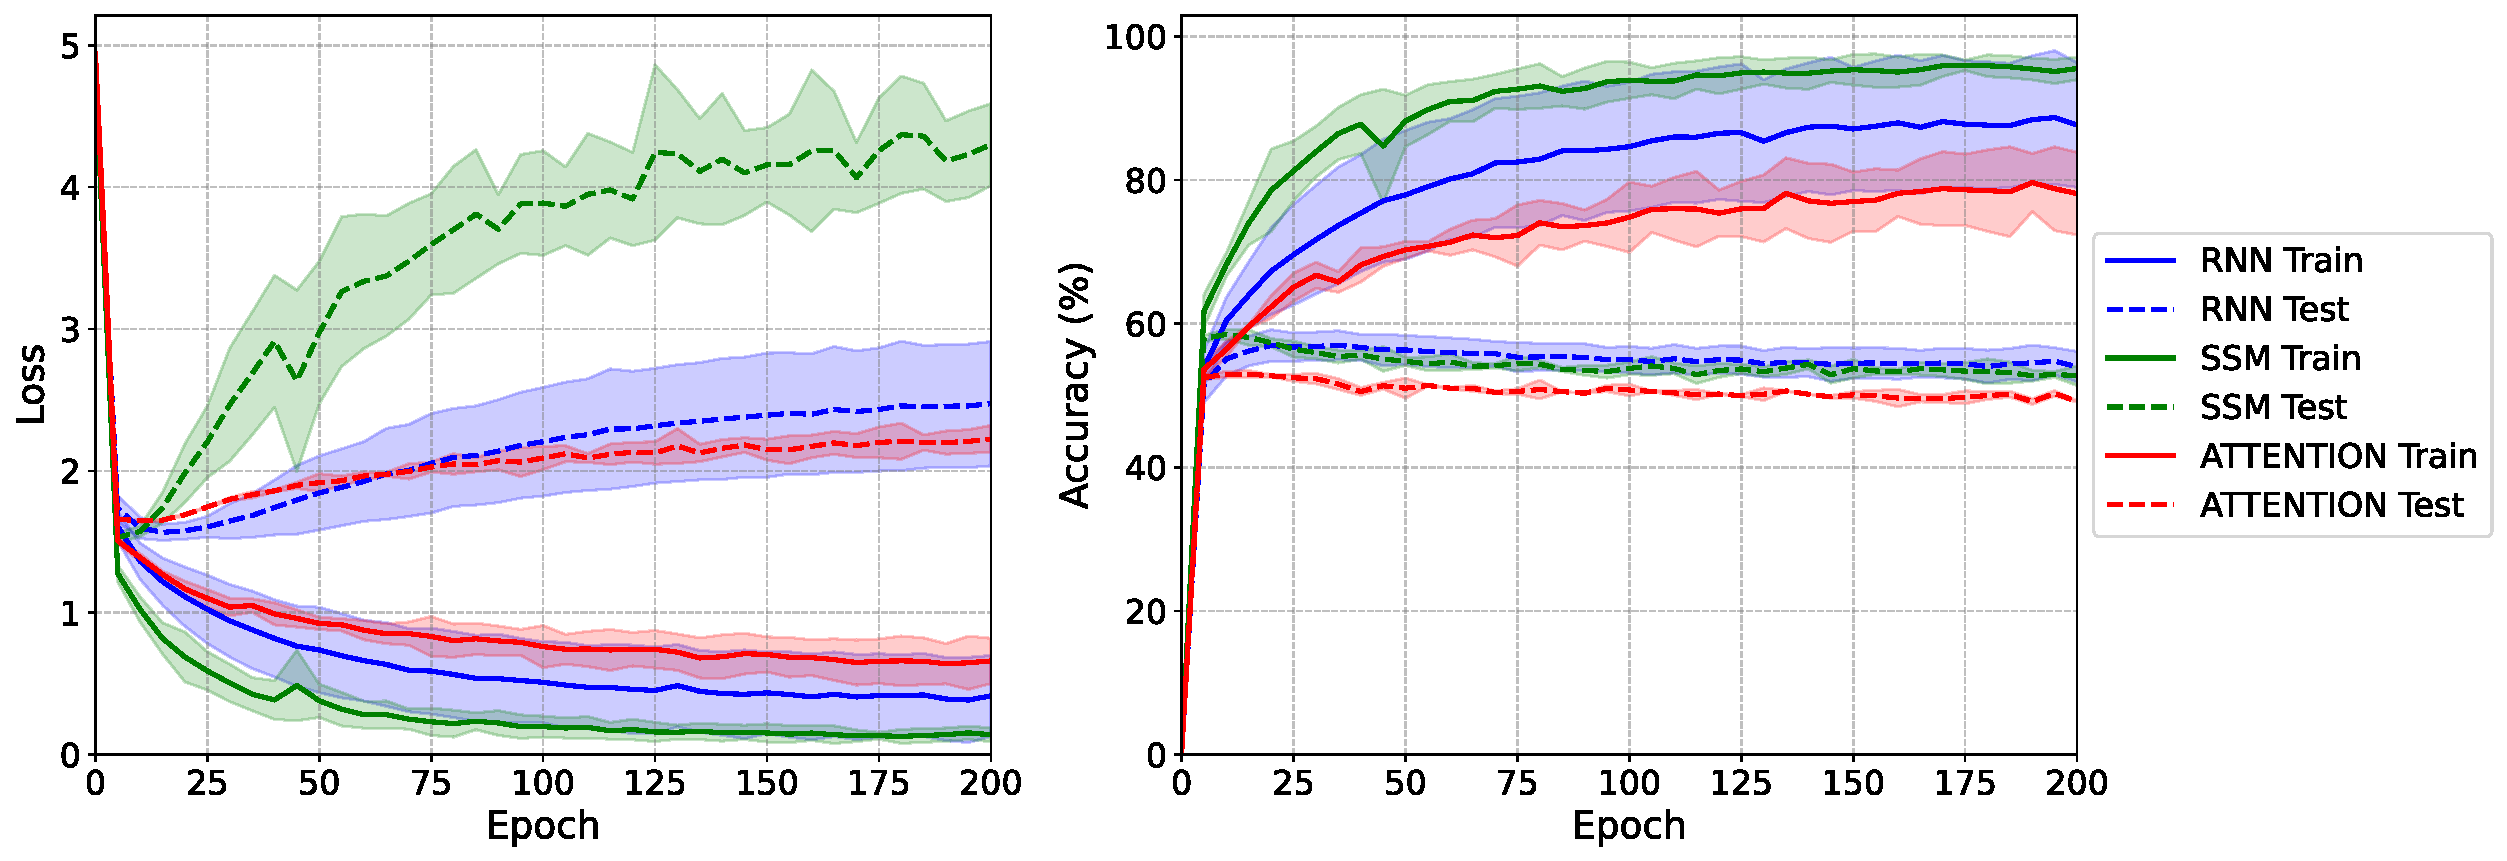
\includegraphics[width=\textwidth]{training_results_embed.pdf}
\caption{Training and validation metrics for RNN, Transformer, and SSM models over 200 epochs.}
\label{fig:training_results}
\end{figure}


\subsection{Comparative Analysis}

Figure \ref{fig:training_results} shows the training and validation metrics for our three model types. The SSM achieved the best scores for loss and accuracy but showed signs of overfitting. The RNN demonstrated more balanced performance, suggesting better generalization to unseen data. The Transformer had the lowest performance, possibly due to the absence of positional encoding. The strong performance of the SSM supports the potential of unified representation for pixel and byte data. However, its tendency to overfit suggests that predicting only the next value might not be sufficient for effective learning in all cases. The balanced performance of the RNN indicates that simpler architectures can still be effective for our task. The Transformer's lower performance suggests that complex attention mechanisms may not always be necessary or beneficial for this type of data.

\subsubsection{Generation Evaluation Metrics}

To assess the effectiveness of our approach and various model architectures, we evaluated their generation capabilities. We tested State Space Models (SSM), Attention models (Att), and Recurrent Neural Networks (RNN) in generating 32 consecutive sequences. Our evaluation used three metrics: Hamming Distance \cite{hamming1950error}, Cosine Similarity, and BLEU Score \cite{papineni2002bleu}.

\begin{table}[ht]
\centering
\small
\begin{tabular}{cccccccccc}
\hline
Type & Dir. & Emb. & Conv. & In Emb & Hidden State & Depth & Hamming & Cosine & BLEU \\
\hline
SSM & Bi & PxBy & Y & 81 & 64 & 1 & 0.170 $\pm$ 0.086 & 0.883 $\pm$ 0.105 & 0.753 $\pm$ 0.115 \\
SSM & Bi & PxBy & Y & 81 & 64 & 2 & 0.158 $\pm$ 0.074 & 0.896 $\pm$ 0.095 & 0.771 $\pm$ 0.097 \\
SSM & Uni & PxBy & Y & 81 & 64 & 2 & 0.166 $\pm$ 0.081 & 0.886 $\pm$ 0.102 & 0.760 $\pm$ 0.106 \\
Att & - & PxBy & Y & 81 & 64 & 1 & 0.157 $\pm$ 0.064 & 0.887 $\pm$ 0.103 & 0.765 $\pm$ 0.088 \\
Att & - & PxBy & Y & 81 & 64 & 2 & 0.159 $\pm$ 0.066 & 0.887 $\pm$ 0.103 & 0.760 $\pm$ 0.092 \\
RNN & Bi & Center & N & 81 & 64 & 2 & 0.185 $\pm$ 0.074 & 0.888 $\pm$ 0.083 & 0.750 $\pm$ 0.093 \\
RNN & Bi & PxBy & Y & 81 & 64 & 2 & 0.153 $\pm$ 0.061 & 0.902 $\pm$ 0.090 & 0.777 $\pm$ 0.083 \\
RNN & Bi & PxBy & Y & 162 & 64 & 2 & 0.152 $\pm$ 0.062 & 0.905 $\pm$ 0.089 & 0.778 $\pm$ 0.084 \\
RNN & Bi & PxBy & Y & 36 & 64 & 2 & 0.152 $\pm$ 0.061 & 0.904 $\pm$ 0.090 & 0.778 $\pm$ 0.083 \\
RNN & Bi & PxBy & Y & 81 & 128 & 2 & 0.153 $\pm$ 0.063 & 0.903 $\pm$ 0.091 & 0.776 $\pm$ 0.086 \\
RNN & Bi & PxBy & Y & 81 & 32 & 2 & \textbf{0.149} $\pm$ 0.062 & 0.899 $\pm$ 0.095 & \textbf{0.785} $\pm$ 0.082 \\
RNN & Bi & PxBy & Y & 81 & 64 & 1 & 0.149 $\pm$ 0.062 & 0.897 $\pm$ 0.096 & 0.780 $\pm$ 0.085 \\
RNN & Bi & PxBy & Y & 81 & 64 & 3 & 0.153 $\pm$ 0.063 & \textbf{0.906} $\pm$ 0.087 & 0.776 $\pm$ 0.086 \\
RNN & Bi & PxBy & N & 81 & 64 & 2 & 0.151 $\pm$ 0.062 & 0.903 $\pm$ 0.090 & 0.779 $\pm$ 0.084 \\
RNN & Uni & PxBy & Y & 81 & 64 & 2 & 0.153 $\pm$ 0.064 & 0.904 $\pm$ 0.088 & 0.777 $\pm$ 0.087 \\
\hline
\end{tabular}
\caption{Comparison of model characteristics and performance (mean $\pm$ std)}
\label{tab:model_comparison}
\end{table}

The results show variations across different model configurations. Among RNN models with PxBy embedding, we observed a Hamming distance of 0.149 $\pm$ 0.062 and a BLEU score of 0.785 $\pm$ 0.082 for a bidirectional model with convolution, 81 embedding dimensions, and 32 hidden state dimensions. The highest cosine similarity (0.906 $\pm$ 0.087) was achieved by a 3-layer RNN model. We noted some differences in performance between models with and without convolution, as well as between unidirectional and bidirectional configurations, though these differences were not always substantial. Changing the embedding dimension (36, 81, 162) in RNN models resulted in similar performance levels. RNN models using center embedding showed different results compared to those using PxBy embedding. The performance of SSM and Attention models varied in comparison to RNN models across the different metrics, but no model type consistently outperformed the others across all measures.

\subsection{Identified Challenges}

Our initial results revealed several limitations in our embedding approach. While we observed variations in performance across different model configurations, the differences were often not substantial \cite{wang2020deep}. The PxBy embedding, which we initially thought promising, did not consistently outperform simpler approaches across all metrics and model types. Based on these findings, we recognized the need to refine our approach. The repetition of sequences in our generated output indicated that our embedding method might not be capturing the full range of patterns in our data \cite{bengio2013representation}.

\section{Optimizing Unified Representation}

\subsection{Refined Embedding Approach}

To address the challenges identified in our initial experiments, we propose a revised embedding strategy. Instead of using a convolutional approach, we now focus on six specific positions within each token, with the input dimension equal to the output dimension. This change allows for a larger embedding size while potentially improving the model's ability to capture relevant patterns. We also recognized the need for a more flexible tokenizer \cite{kudo2018sentencepiece}. Our initial implementation became cumbersome when generating new data, highlighting the importance of a more versatile approach. We are exploring ways to integrate all necessary functionality into the tokenizer itself, which should simplify our overall pipeline and potentially improve performance. These refinements reflect a shift from our initial exploration towards a more focused approach to unified representation. While our initial results provided valuable insights, they also revealed the complexities inherent in multimodal sequence modeling and the need for continuous iteration in our methods \cite{lecun2015deep}.

\subsubsection{Dataset Construction}

\sloppy

For our refined approach, we created a new dataset combining images, text, and audio extracted from Pokemon sprite animations. This dataset, available at \url{https://huggingface.co/datasets/ffurfaro/PixelBytes-PokemonAll}, was compiled through web scraping of Pokepedia and includes descriptions of the Pokemon along with their associated cries. The dataset consists of animated, pixelated GIFs of Pokemon sprites as the visual component. The audio files are two-channel recordings: Channel 1 contains the original mono sound of the Pokemon cry, while Channel 2 features a filtered version simulating a bits Game Boy speaker output to verify our approach for control problems. This setup allows us to model a simplified dynamic physical system, where the original sound acts as the "action" input and the filtered output represents the "state" of the system. The transfer function of this bandpass filter can be approximated as:

\begin{equation}
H(s) = \frac{K \omega_n^2}{s^2 + 2\zeta\omega_n s + \omega_n^2}
\end{equation}

where $K$ is the gain, $\omega_n$ is the natural frequency, and $\zeta$ is the damping ratio. These parameters can be adjusted to closely match the frequency response of a Game Boy speaker.

\subsection{Enhanced Tokenization Strategy}

Building on our previous work, we developed an improved tokenization strategy using the ActionPixelBytesTokenizer. This tokenizer aims to handle multimodal data more effectively, including text, images, and audio, while maintaining a unified representation. The tokenizer employs a combined vocabulary that includes ASCII bytes, RGB values from the NES palette, and action states for control and audio. This approach attempts to create a consistent representation across different data types. For text processing, the tokenizer converts to lowercase ASCII bytes. Images are converted to Lab color space and quantized to the nearest NES palette color. Audio data is normalized and mapped to predefined action states, were setpoint is reset to zero (standard equilibrium). All token numbers are now 151, where index 0 corresponds to the null padding value, and indices 1 and 2 are transition values. A key aspect of the new tokenizer is its sequence construction method. Instead of using convolutional methods, we focus on six specific positions for each token for no repetition in sequencing of 3D zigzag scheme (Figure \ref{fig:approach_overview}). This approach creates context-target pairs that aim to capture relationships between neighboring tokens in both space and time. The sequence construction algorithm is detailed below:

\begin{algorithm}[ht]
\small  % \footnotesize
\caption{Create Sequence Data
\newline
\textbf{Input:} $\mathbf{X} \in \mathbb{R}^{T \times H \times W}$: context array
\newline
\textbf{Output:} $\mathbf{C} \in \mathbb{R}^{THW \times 6}$: context, $\mathbf{Y} \in \mathbb{R}^{THW \times 1}$: targets
\newline
\textbf{Note:} $T$: time steps, $H$: height, $W$: width
}
\begin{algorithmic}[0]
\State \textbf{Initialize:} $\mathbf{P} \in \mathbb{R}^{(T+1) \times (H+2) \times (W+2)}$ as padded array
\Function{CreateSequenceData}{$\mathbf{X}$}
    \State $\mathbf{P} \gets \text{Pad}(\mathbf{X}, (1,1,1,1,1,0), \text{mode='constant'}, \text{value=0})$
    \State $\mathbf{S}_1 \gets \mathbf{P}_{1:T, 1:H, 2:W+1}$
    \State $\mathbf{S}_2 \gets \mathbf{P}_{1:T, 2:H+1, 2:W+1}$
    \State $\mathbf{S}_3 \gets \mathbf{P}_{1:T, 3:H+2, 2:W+1}$
    \State $\mathbf{S}_4 \gets \mathbf{P}_{2:T+1, 1:H, 1:W}$
    \State $\mathbf{S}_5 \gets \mathbf{P}_{2:T+1, 1:H, 2:W+1}$
    \State $\mathbf{S}_6 \gets \mathbf{P}_{2:T+1, 2:H+1, 1:W}$
    \State $\mathbf{C} \gets \text{Stack}([\mathbf{S}_1, \mathbf{S}_2, \mathbf{S}_3, \mathbf{S}_4, \mathbf{S}_5, \mathbf{S}_6], \text{dim=-1})$
    \State $\mathbf{C} \gets \text{Reshape}(\mathbf{C}, [THW, 6])$
    \State $\mathbf{Y} \gets \text{Reshape}(\mathbf{X}, [THW, 1])$
    \For{$i \gets 2$ \textbf{to} $THW$}
        \State $\mathbf{C}_{i,6} \gets \mathbf{Y}_{i-1,1}$
    \EndFor
    \State \Return $\mathbf{C}, \mathbf{Y}$
\EndFunction
\end{algorithmic}
\end{algorithm}

This algorithm constructs a context array for sequence modeling. It pads the input to handle boundary conditions and extracts six slices to represent spatial and temporal relationships. The context array $\mathbf{C}$ is formed by stacking these slices, while the targets $\mathbf{Y}$ are derived from the input. The last column of $\mathbf{C}$ is set to the true previous value, implementing an autoregressive feature. The tokenizer is designed to handle various input combinations and includes functionalities such as special token handling and padding.

\subsection{Autoregressive Model Architecture}

Building upon our previous findings in our initial approach, we developed the aPxBySequenceModel architecture. This new architecture is designed to handle both predictive and autoregressive tasks using a Long Short-Term Memory (LSTM) network. The model consists of three main components: an embedding layer, an LSTM sequence model, and a fully connected output layer. The embedding layer maps input tokens to a continuous vector space, with the embedding size calculated based on the input dimension. Specifically, the embedding size is determined by dividing the overall embedding size by the number of positions we focus on within each token. This approach aligns with our revised embedding strategy, which emphasizes six specific positions within each token (with padding 0 to not influence training). The LSTM layer, aims to capture temporal dependencies in the sequence data, potentially improving pattern recognition across different modalities. The model operates in two distinct modes:

\begin{itemize}
    \item \underline{Predictive mode:} In this configuration, the model takes six input values and attempts to predict only the next token.

    \item \underline{Autoregressive mode:} Here, the model's output dimension matches the input dimension (Figure \ref{fig:approach_overview}). Additionally, the output is restructured by multiplying it with the vocabulary size, allowing the model to generate sequences based on the learned representations.
\end{itemize}

During the forward pass, input data is processed through the embedding layer, then through the LSTM layers, and finally through the fully connected layer. The output shape is adjusted based on the operating mode, which may provide the flexibility we found lacking in our initial implementation.

\subsubsection{Model Training and Data Management}

For data management, we developed the \texttt{TokenPxByDataset} class to handle multimodal inputs, including text, image, and audio data. This class generates overlapping sequences from longer inputs, which helps the model capture context across sequence boundaries. It optimizes memory usage through on-the-fly data retrieval, preparing samples only as they are needed. Additionally, the class ensures consistent sequence lengths by implementing circular padding for sequences that extend beyond the end of an item. These features enable efficient processing of variable-length inputs during training.

Our training process includes several improvements to enhance efficiency and monitoring. In the \texttt{\_process\_epoch} function, we manage both autoregressive and non-autoregressive modes. In autoregressive mode, we reshape the input and output sequences, using the input sequence as the target. For non-autoregressive mode, we flatten the outputs and use the provided labels as the target. This flexibility allows the model to adapt to different tasks. The \texttt{train\_model} function alternates between training and validation phases, allowing us to evaluate the model's performance regularly. We use gradient accumulation to simulate larger batch sizes, which helps when GPU memory is limited. The training loop tracks both training and validation metrics (loss and accuracy) for each epoch and saves these metrics to a CSV file. We also implement model checkpointing to keep the best model based on validation loss.

\subsection{Performance Evaluation}

We evaluated three LSTM models: one in predictive mode and two in autoregressive mode, each with approximately 4 million parameters. The models were trained on Kaggle using T4 GPUs. We used an embedding size of 128, a hidden size of 512, and two layers. Training was conducted for 100 epochs with a batch size of 32, a learning rate of 0.001, and a sequence length of 1024.

\subsubsection{Results Comparison}

To manage data proportions, we applied different reduction strategies for image and audio data. This was particularly important for audio data in the autoregressive mode, as it contains more null values to predict, which could potentially hinder training. Table \ref{tab:model_comparison_lstm} presents the final performance metrics after training.

\begin{table}[ht]
\centering
\caption{Comparison of model performance after 100 epochs}
\label{tab:model_comparison_lstm}
\begin{tabular}{|l|c|c|c|c|}
\hline
\textbf{Model} & \textbf{Train Loss} & \textbf{Train Accuracy} & \textbf{Val Loss} & \textbf{Val Accuracy} \\
\hline
Autoregressive (2,2) & 0.2211 & 0.9329 & 0.4519 & 0.8852 \\
Autoregressive (4,2) & 0.2346 & 0.9290 & 0.4914 & 0.8726 \\
Predictive (2,2) & 0.8810 & 0.7440 & 2.1144 & 0.6009 \\
\hline
\end{tabular}
\end{table}

The numbers in parentheses indicate the reduction factors for (audio, image) data. Lower loss and higher accuracy indicate better performance. Both autoregressive models performed better than the predictive model in terms of accuracy and loss on both training and validation sets. The autoregressive model with balanced reduction (2,2) achieved slightly better results than the one with more aggressive audio reduction (4,2). Although the predictive model had lower performance overall, it still reached reasonable accuracy given the complexity of the task. This suggests that our pixelbyte representation is effective, especially when using autoregressive learning.

\begin{figure}[ht]
\centering
\includegraphics[width=\textwidth]{apxby_gen_comparison.png}
\caption{Generation results for the 1st Generation Starter Pokémon using the autoregressive model with a temperature of 0.1. Reference images and generated images are paired sequentially.}
\label{fig:generation_results}
\end{figure}

The complete frame generation results, as shown in Figure \ref{fig:generation_results}, demonstrate spatial consistency in image creation, despite the model being unidirectional. This suggests that data representation may be more crucial than the architecture itself, aligning with recent findings in multimodal learning \cite{baltruvsaitis2018multimodal}. The generated images show coherence in colors and sizes, indicating that the model has captured some key visual features. While our model does not match the image quality of state-of-the-art diffusion models \cite{dhariwal2021diffusion}, it demonstrates the capability to capture multiple modalities (image, text, audio) within a single framework. This aligns with recent trends in multimodal co-learning \cite{liang2022mind}, although further optimization is needed to improve generation quality. The trained models are available at \url{https://huggingface.co/ffurfaro/aPixelBytes-Pokemon} for further examination and replication of our results.

\section{Discussion and Future Directions}

Our experiments with various model architectures for unified text and image generation have led to unexpected insights and a shift in our approach. Initially, we explored bidirectional RNN models using PixelBytes (PxBy) embedding with convolutional layers, anticipating improved multimodal data representation. However, deeper analysis revealed limitations in this approach and these findings have led us to reconsider our tokenizer design. 

Our next results with LSTM models have been particularly enlightening. The autoregressive models significantly outperformed the predictive model, suggesting that maintaining equal input and output dimensions is important for our task. This aligns with recent research emphasizing the importance of preserving structural information in multimodal embeddings \cite{verHo2021efficient}. The performance difference between the two autoregressive models highlights the impact of data balancing strategies. The model with balanced reduction (2,2) for audio and image data showed slightly better results, indicating that can be overfitting with animated image. We now aim for a more versatile solution that can handle all aspects of data preparation and support true autoregressive modeling. Our \texttt{TokenPxByDataset} class remains valuable, but we are working to integrate its functionality more closely with our revised tokenizer for a more streamlined data pipeline.

While we initially explored both RNN and State Space Models (SSM), with SSMs showing promising rapid convergence \cite{dao2024transformers}, our focus has shifted towards simplifying the overall architecture. Our approach offers an alternative to the principles of models like ImageBind \cite{girdhar2023imagebind}, as our preliminary results suggest it may be possible to unify modalities without relying on intermediate representations. We now recognize the potential benefits of allowing emergent properties to develop within a simplified framework. Moving forward, we will refine our strategy to better utilize specific input positions for high-definition image and sound. We also aim to further simplify our model architecture to promote the emergence of natural multimodal representations. Additionally, we plan to explore alternative approaches like Diffusion-LM \cite{li2022diffusion}, which may offer new perspectives on multimodal sequence modeling. While our work is still in progress, it aligns with recent trends in multimodal AI research \cite{baltruvsaitis2018multimodal} and could potentially provide a versatile base for various multimodal tasks.

\bibliographystyle{plain}
\bibliography{references}

\end{document}
